\documentclass{template}

\title{MA 580 Assignment 1}
\author{Kyle Hansen}
\date{5 September 2025}

\usepackage{cancel}



\begin{document}

\maketitle

\section{}

Given any vector norm $\vert \vert \cdot\vert \vert $ on $\mathbb{C}^n$:

\subsection{}

Show that

\begin{equation}\label{eq:question1a}
    \left\vert \vert \vert x\vert \vert  - \vert \vert y\vert \vert  \right\vert  \leq \vert \vert x-y\vert \vert ;\quad \forall \:  x,y \in \mathbb{C}^n
\end{equation}

Using the definition of a vector norm $\vert \vert \cdot\vert \vert $:

\begin{enumerate}[label=(\alph*)]
    \item\label{item1} $\vert \vert x\vert \vert  \geq 0$ for all $x\in \mathbb{C}$; $\vert \vert x\vert \vert =0 \iff x=0$
    \item\label{item2} $\vert \vert x+y\vert \vert  \leq \vert \vert x\vert \vert +\vert \vert y\vert \vert $
    \item\label{item3} $\vert\vert cx|| = \vert c\vert\times\vert\vert x\vert \vert$ for all $c\in \mathbb{C}$
\end{enumerate}

From \ref{item1}:

\begin{equation}\label{eq:firstcase}
    || (x-y)+y || \leq || (x-y)|| + || y ||
\end{equation}

or 

\begin{equation}
    || (x-y)+y || - || y || \leq || (x-y)|| 
\end{equation}
\begin{equation}
    || x || - || y || \leq || x-y|| 
\end{equation}

which satisfies \autoref{eq:question1a} for $||x|| \geq ||y||$ (when the L.H.S. is positive), but does not account for $||y|| > ||x||$, when the absolute value of the LHS may be greater than the RHS. This case may be shown starting from \ref{item2}:

\begin{equation}
    ||x-y|| = |-1|\;||(y-x)|| = ||(y-x)||
\end{equation}

then, similarly to \autoref{eq:firstcase},

\begin{equation}
    || (y-x)+x || \leq || (y-x)|| + || x ||
\end{equation}
\begin{equation*}
    \vdots
\end{equation*}
\begin{equation}
    || y || - || x || \leq || y-x|| = ||x-y|| 
\end{equation}

Then, since 

\begin{equation}
    \pm(|| x || - || y ||) \leq || x-y|| 
\end{equation}

or

\begin{equation}
    |\;||x|| - ||y||\;| \leq||x-y||
\end{equation}

\subsection{}

Given the function $f:\mathbb{C}^n \rightarrow \mathbb{C}^n$ defined by $f(x) = \mathbf{A}x$ where $\mathbf{A}\in \mathbb{C}^{n\times n}$ is a fixed matrix. Show $f$ is continuous.

For $f$ to be continuous, $||f(x_n)-f(x)||\rightarrow 0$ for every sequence $\{x_n\}$ that converges to $x$. 

Since matrix operations are linear (and thus additive), 

\begin{equation}
    \norm{\mathbf{A}x_n - \mathbf{A}x} = \norm{\mathbf{A}(x_n - x)}
\end{equation}

By Fact 2.18 in \cite{ipsen2009numerical} and \autoref{item1} in the definition of a norm:

\begin{equation}\label{eq:norm-multiplication}
    0 \leq \norm{\mathbf{A}(x_n - x)} \leq \norm{\mathbf{A}} \norm{(x_n - x)}
\end{equation}

By the definition of a Cauchy sequence, $\norm{(x_n - x)} \rightarrow 0$. Since $\norm{\mathbf{A}}$ is a constant, the right hand side of \autoref{eq:norm-multiplication} then also converges to zero. Since the left hand side is non-negative and less than the right hand side, it also converges to zero:

\begin{equation}
    \norm{\mathbf{A}(x_n - x)} \rightarrow 0
\end{equation}

and thus the function $f(x)$ is continuous.

\subsection{}

Let $\ip{\cdot}{\cdot}$ be an inner product on $\C^n$. Define the function $f:\C^n \to \C$ by $f(\vec{x}) = \ip{\vec{x}}{\vec{u}}$, where  $\vec{u} \in \C^n$ if a fixed vector. Show $f$ is continuous.

An inner product is defined as $\left<\cdot,\cdot\right> : V\times V \rightarrow \mathbb{K}$ such that:

\begin{enumerate}[label=(\roman*)]
    \item\label{item:positive-definite} $\left<x,x\right> \geq 0 \quad \forall \: x \in V$; \qquad $\ip{x}{x} = 0 \iff x=0$
    \item\label{item:linearity} $\left<u+v, w\right> = \left<u, w\right> + \left<v, w\right>$
    \item\label{item:scalability} $\left<\lambda u, v\right> = \lambda\left<u, v \right>$
    \item\label{item:conjugate-symm} $\ip{u}{v} = \overline{\ip{v}{u}}$
\end{enumerate}

Then, by \autoref{item:linearity}, 

\begin{equation}
    \ip{x_n}{u} - \ip{x}{u} = \ip{(x_n - x)}{u}
\end{equation}

By the Cauchy-Schwarz inequality, 

\begin{equation}\label{eq:cauchy-inequality}
      |{\ip{(x_n - x)}{u}}| \leq \norm{(x_n - x)}\times\norm{u}
\end{equation}

By the definition of a Cauchy Sequence converging to $x$, $\norm{(x_n - x)}\rightarrow 0$. Then the RHS of \autoref{eq:cauchy-inequality} also converges to zero. Since $\text{LHS}\leq\text{RHS}$, the LHS must also converge to zero, and thus

\begin{equation}
      |{\ip{(x_n - x)}{u}}| \rightarrow 0
\end{equation}

Then, by \autoref{item:linearity} and \autoref{item:scalability}, an equivalent statement is:

\begin{equation}
    |\ip{x_n}{u} - \ip{x}{u}| \rightarrow 0
\end{equation}

or

\begin{equation}
    |f(x_n) - f(x)| \rightarrow 0
\end{equation}

and thus the function is continuous.

\newpage
\section{}

Let $(V, \ip{\cdot}{\cdot})$ be a $n$-dimensional inner product space, over $\mathbb{K} = \R \text{ or } \C$, equipped with the  norm $\norm{x} = \ip{x}{x}^{1/2}$. Let $\{v_i\}_{i=1}^n$ be an orthonormal basis for $V$, i.e., $\ip{v_i}{v_j} = \delta_{ij}$, $i, j \in \{1, \ldots, n\}$.

\subsection{}\label{sec:fourier-expansion}

Show that any $x \in V$ can be written as the linear combination, $x = \sum_{i = 1}^n \xi_i v_i$ with $\xi_i = \ip{x}{v_i}$ (Fourier Expansion of $x$).

Assume that $x$ can be expanded as a linear combination of the basis vectors:

\begin{equation}
    x = \sum_{i=1}^n x_i = \sum_{i=1}^n a_i v_i
\end{equation}

Where  $x_i$ is the component of $x$ in the $v_i$ direction, with a scalar magnitude of $a_i$. This projection always exists and is unique. Then

\begin{equation}
    v_i = \frac{1}{a_i} x_i
\end{equation}

The definition of the orthonormal basis can then be rewritten:

\begin{equation}
    \ip{\frac{1}{a_i} x_i}{v_j} = \delta_{ij}
\end{equation}
\begin{equation}
    \ip{x_i}{v_j} = \delta_{ij}a_i
\end{equation}

then the coefficients are given by

\begin{equation}
    a_i = \ip{x_i}{v_i} = \xi_i
\end{equation}

The coefficient $\xi_i$ is always defined and is unique, so $x$ may always be expanded uniquely in this way.



\subsection{}

Show that for $x \in V$, $\norm{x}^2 = \sum_{i = 1}^n |\ip{x}{v_i}|^2$. This is known as Parseval's identity.



From the problem definition,

\begin{equation}
    \norm{x}^2 = \ip{x}{x}
\end{equation}

Following \autoref{sec:fourier-expansion}, this can then be rewritten as

\begin{equation}
    \norm{x}^2 = \ip{\sum_{i=1}^n \xi_i v_i}{\sum_{j=1}^n \xi_j v_j}
\end{equation}

This term can be simplified using another inner product property implicit in \autoref{item:scalability} and \autoref{item:conjugate-symm}:

\begin{equation}
    \norm{x}^2 = \sum_{i=1}^n \sum_{j=1}^n \xi_i \overline{\xi_j}\ip{v_i}{v_j}
\end{equation}

Since the set of basis vectors $\{v\}$ are orthonormal (by the problem definition), this can further simplify, as all terms where $i\neq j$ become zero, and the inner product $\ip{v_i}{v_j}$ becomes 1 for all terms where $i=j$:

\begin{equation}
    \norm{x}^2 = \sum_{i=1}^n \xi_i \overline{\xi_i}
\end{equation}

And, using a property of the complex conjugate,

\begin{equation}
    \norm{x}^2 = \sum_{i=1}^n |\xi_i|^2
\end{equation}

Where $\xi_i = \ip{x}{v_i}$:

\begin{equation}
    \norm{x}^2 = \sum_{i=1}^n |\ip{x}{v_i}|^2
\end{equation}

\newpage
\section{}

Consider the vector norms $\norm{\cdot}_1$, 
$\norm{\cdot}_2$, $\norm{\cdot}_\infty$ on $\R^n$ and their induced matrix norms. 



\subsection{}\label{sec:l2_vec_inequalities}

Show that for all $\vec{x} \in \R^n$,
\[
\norm{\vec{x}}_\infty \leq \norm{\vec{x}}_2 \leq \norm{\vec{x}}_1 \leq \sqrt{n}\norm{\vec{x}}_2 \leq n \norm{\vec{x}}_\infty.
\]

The first inequality can be proven intuitively; since $\norm{\vec{x}}_\infty = \max_{i=1\dots n} (|x_i|) = \sqrt{\max(x_i^2)}$. The L2 norm is defined as:

\begin{equation}
    \norm{\vec{x}}_2 = \sqrt{\sum_{i=1}^n (x_i)^2}
\end{equation}

Since all terms $x_i^2$ are non-negative, it is certain that $\max (x_i^2) \leq\sum x_i^2$, and $\sqrt{\max (x_i^2)} \leq\sqrt{\sum x_i^2}$. Thus

\begin{equation}\label{eq:first_norm_inequality}
    \norm{\vec{x}}_\infty \leq \norm{\vec{x}}_2.
\end{equation}

\hrule

The L2 norm can be re-written:

\begin{equation}
    \norm{\vec{x}}_2^2 = \sum_{i=1}^n (x_i^2) = \norm{\vec{x}^\top\vec{x}}_1
\end{equation}

and by the Cauchy-Schwarz inequality,

\begin{equation}
    \norm{\vec{x}^\top\vec{x}}_1 \leq \norm{\vec{x}^\top}_1 \cdot \norm{\vec{x}}_1 = \norm{\vec{x}}_1^2
\end{equation}

Then

\begin{equation}
    \norm{\vec{x}}_2^2 \leq \norm{\vec{x}}_1^2
\end{equation}

or

\begin{equation}\label{eq:second_norm_inequality}
    \norm{\vec{x}}_2 \leq \norm{\vec{x}}_1
\end{equation}

\hrule

Using the Cauchy-Schwarz inequality, 

\begin{equation}
    \norm{\vec{x}}_1 = \sum_{i=1}^n (x_i\cdot 1) = \ip{x}{\vec{1}} \leq \sqrt{\ip{\vec{x}}{\vec{x}} \ip{\vec{1}}{\vec{1}}}
\end{equation}

and since $\sqrt{\ip{\vec{x}}{\vec{x}}} = \norm{\vec{x}}_2$ and $\ip{\vec{1}}{\vec{1}} = n$,

\begin{equation}\label{eq:third_norm_inequality}
    \norm{\vec{x}}_1 \leq \sqrt{n}\norm{\vec{x}}_2
\end{equation}

\hrule

The fourth term of the inequality in the problem definition can be rewritten

\begin{equation}\label{eq:l-2}
    \left( \sqrt{n} \norm{\vec{x}}_2    \right)^2 = n\sum_{i=1}^n x_i^2
\end{equation}

And the last term in the inequality can be rewritten in a similar way:

\begin{equation}\label{eq:l-inf}
    \left( n \norm{\vec{x}}_\infty\right)^2 = n^2(\max(|x_i|))^2     = n(n\max(x_i^2)) = n\sum_{i=1}^n \max(x_i^2)
\end{equation}

And, since all terms $x_i^2$ are less than or equal to $\max(x_i^2)$, the sum in \autoref{eq:l-2} must be less than the sum in \autoref{eq:l-inf}, and thus

\begin{equation}
    \left( \sqrt{n} \norm{\vec{x}}_2    \right)^2 \leq \left( n \norm{\vec{x}}_\infty\right)^2
\end{equation}

or

\begin{equation}\label{eq:fourth_norm_inequality}
    \sqrt{n}\norm{\vec{x}}_2 \leq n \norm{\vec{x}}_\infty
\end{equation}

Combining Equations \ref{eq:first_norm_inequality}, \ref{eq:second_norm_inequality}, \ref{eq:third_norm_inequality}, and \ref{eq:fourth_norm_inequality} yields the original inequality from the problem definition,

\begin{equation}
    \norm{\vec{x}}_\infty \leq \norm{\vec{x}}_2 \leq \norm{\vec{x}}_1 \leq \sqrt{n}\norm{\vec{x}}_2 \leq n \norm{\vec{x}}_\infty.
\end{equation}




\subsection{}

Use the result of the previous part to show
that for all $\mat{A} \in \R^{n\times n}$, 
\[
    \norm{\mat{A}}_1 \leq \sqrt{n} \norm{\mat{A}}_2 \leq n \norm{\mat{A}}_1 \quad \text{and } \quad 
    \norm{\mat{A}}_\infty \leq \sqrt{n} \norm{\mat{A}}_2 \leq n \norm{\mat{A}}_\infty. 
\]

By the previous part, for any $\vec{x} \in \R^n$,

\begin{equation}
    \norm{\mat{A}\vec{x}}_1 \leq \sqrt{n}\norm{\mat{A}\vec{x}}_2
\end{equation}

By submultiplicativaty,

\begin{equation}
    \norm{\mat{A}\vec{x}}_1 \leq \sqrt{n}\norm{\mat{A}}_2\norm{\vec{x}}_2
\end{equation}

Let $\norm{\vec{x}}_1 = 1$. Again, using the result of the previous part, $\norm{\vec{x}}_2 \leq \norm{\vec{x}}_1 = 1$:

\begin{equation}\label{eq:A1_leq_sqnA2}
    \norm{\mat{A}}_1 \leq \sqrt{n}\norm{\mat{A}}_2\norm{\vec{x}}_2 \leq \sqrt{n}\norm{\mat{A}}_2\cancelto{1}{\norm{\vec{x}}_1}
\end{equation}

The next portion of the inequality can be proved in a similar way. By the previous part, for any $\vec{x} \in \R^n$,

\begin{equation}
    \norm{\mat{A}\vec{x}}_2 \leq \norm{\mat{A}\vec{x}}_1
\end{equation}

By the submultiplicative property, $\norm{\mat{A}\vec{x}}_1 \leq \norm{\mat{A}}_1\norm{\vec{x}}_1$, so 

\begin{equation}
    \norm{\mat{A}\vec{x}}_2 \leq \norm{\mat{A}}_1\norm{\vec{x}}_1
\end{equation}

By the inequality in the previous part, $\norm{\vec{x}}_1 \leq \sqrt{n}\norm{\vec{x}}_2$, so 

\begin{equation}
    \norm{\mat{A}\vec{x}}_2 \leq \norm{\mat{A}}_1\sqrt{n}\norm{\vec{x}}_2
\end{equation}

Letting $\norm{\vec{x}}_2 = 1$, this gives:

\begin{equation}
    \norm{\mat{A}}_2 \leq \sqrt{n}\norm{\mat{A}}_1
\end{equation}

Multiplying this statement by $\sqrt{n}$ yields

\begin{equation}\label{eq:A2_leq_sqnA1}
    \sqrt{n}\norm{\mat{A}}_2 \leq n\norm{\mat{A}}_1
\end{equation}

Combining \autoref{eq:A1_leq_sqnA2} and \autoref{eq:A2_leq_sqnA1} yields the first inequality in the problem definition: $ \norm{\mat{A}}_1 \leq \sqrt{n} \norm{\mat{A}}_2 \leq n \norm{\mat{A}}_1$. 

\hrule

The second statement in the problem definition is proven in a similar way. From the previous part, for any $\vec{x} \in \R^n$,

\begin{equation}
    \norm{\mat{A}\vec{x}}_\infty \leq \norm{\mat{A}\vec{x}}_2
\end{equation}

By submultiplicativity, $\norm{\mat{A}\vec{x}}_2 \leq \norm{\mat{A}}_2\norm{\vec{x}}_2$, so 

\begin{equation}
    \norm{\mat{A}\vec{x}}_\infty \leq \norm{\mat{A}}_2\norm{\vec{x}}_2
\end{equation}

From the previous part, $\sqrt{n}\norm{\vec{x}}_2 \leq n\norm{\vec{x}}_\infty$, or $\norm{\vec{x}}_2 \leq \sqrt{n}\norm{\vec{x}}_\infty$, so

\begin{equation}
    \norm{\mat{A}\vec{x}}_\infty \leq \norm{\mat{A}}_2\sqrt{n}\norm{\vec{x}}_\infty
\end{equation}

Then, letting $\norm{\vec{x}}_\infty = 1$, it can be shown that

\begin{equation}\label{eq:Ainf_leq_sqrnA2}
    \norm{\mat{A}}_\infty \leq \sqrt{n}\norm{\mat{A}}_2
\end{equation}

Thus proving the first portion of the second inequality in the problem definition. The second portion can be proven in a similar way. For any $\vec{x} \in \R^n$,

\begin{equation}
    \sqrt{n}\norm{\mat{A}\vec{x}}_2 \leq n\norm{\mat{A}\vec{x}}_\infty
\end{equation}

By submultiplicativity, $\norm{\mat{A}\vec{x}}_\infty \leq \norm{\mat{A}}_\infty\norm{\vec{x}}_\infty$, so

\begin{equation}
    \sqrt{n}\norm{\mat{A}\vec{x}}_2 \leq n\norm{\mat{A}}_\infty\norm{\vec{x}}_\infty
\end{equation}

By the inequality in the previous part, $\norm{\vec{x}}_\infty \leq \norm{\vec{x}}_2$, so

\begin{equation}
    \sqrt{n}\norm{\mat{A}\vec{x}}_2 \leq n\norm{\mat{A}}_\infty\norm{\vec{x}}_2
\end{equation}

Letting $\norm{\vec{x}}_2 = 1$, 

\begin{equation}\label{eq:sqnA2_leq_nA_infty}
    \sqrt{n}\norm{\mat{A}}_2 \leq n\norm{\mat{A}}_\infty
\end{equation}

Then from \autoref{eq:A1_leq_sqnA2}, \ref{eq:A2_leq_sqnA1} \ref{eq:Ainf_leq_sqrnA2}, and \ref{eq:sqnA2_leq_nA_infty}, 

\begin{equation}
    \norm{\mat{A}}_1 \leq \sqrt{n} \norm{\mat{A}}_2 \leq n \norm{\mat{A}}_1 \quad \text{and } \quad 
    \norm{\mat{A}}_\infty \leq \sqrt{n} \norm{\mat{A}}_2 \leq n \norm{\mat{A}}_\infty.
\end{equation}


\newpage
\section{}

Let $\mat{A} \in \R^{n \times n}$ be symmetric with eigenvalues
$\lambda_1 \leq \lambda_2 \leq \cdots \leq \lambda_n$.

\subsection{}

Show that,
$\lambda_1 \vec{x}^\top \vec{x} \leq \vec{x}^\top \mat{A} \vec{x} \leq  \lambda_n \vec{x}^\top \vec{x}$, for all $\vec{x} \in \R^n$.

Since $\mat{A}$ is real and symmetric, by the spectral theorem for real symmetric matrices, there exists a matrix $\mat{U}$ such that $\mat{A} = \mat{U}\mat{\Lambda}\mat{U}^\top$, where $\mat{\Lambda}$ is a diagonal matrix composed of the eigenvalues of $\mat{A}$, and $\mat{U}$ is orthogonal and composed of the eigenvectors of $\mat{A}$.

Since $\mat{U}$ is orthonormal, it has the useful property that $\mat{U}^\top = \mat{U}^{-1}$, or $\mat{U}^\top\mat{U} = \mat{I}$.

Since $\mat{A} = \mat{U}\mat{\Lambda}\mat{U}^\top$, it is also true that:

\begin{equation}
    \vec{x}^\top\mat{A}\vec{x} = \vec{x}^\top\mat{U}\mat{\Lambda}\mat{U}^\top\vec{x}
\end{equation}
\begin{equation}
    \vec{x}^\top\mat{A}\vec{x} = (\mat{U}^\top\vec{x})^\top\mat{\Lambda}\mat{U}^\top\vec{x}
\end{equation}

or

\begin{equation}\label{eq:middle-term}
    \vec{x}^\top\mat{A}\vec{x} = \sum_{i=1}^n \lambda_i (\mat{U}^\top\vec{x})_i^2
\end{equation}

The term $\vec{x}^\top \vec{x}$ can be rewritten using $\mat{U}^\top\mat{U} = \mat{I}$:

\begin{equation}
    \vec{x}^\top \vec{x} = \vec{x}^\top \mat{I} \vec{x} = \vec{x}^\top\mat{U}\mat{U}^\top \vec{x} = (\mat{U}^\top \vec{x})^\top\mat{U}^\top \vec{x}
\end{equation}
\begin{equation}\label{eq:end-terms}
     \vec{x}^\top \vec{x} = \sum_{i=1}^n (\mat{U}^\top\vec{x})_i^2
\end{equation}



\hrule



Implicit from the inequality in the problem definition is:

\begin{equation}
    \sum_{i=1}^n \lambda_1 \leq \sum_{i=1}^n \lambda_i \leq \sum_{i=1}^n \lambda_n
\end{equation}

Multiplying this inequality by $(\mat{U}^\top\vec{x})_i^2$ (and factoring out the constant $\lambda$ terms) gives:

\begin{equation}
     \lambda_1 \sum_{i=1}^n(\mat{U}^\top\vec{x})_i^2\leq \sum_{i=1}^n \lambda_i(\mat{U}^\top\vec{x})_i^2 \leq\lambda_n \sum_{i=1}^n (\mat{U}^\top\vec{x})_i^2
\end{equation}

Which can be rewritten using \autoref{eq:middle-term} and \autoref{eq:end-terms} as:

\begin{equation}
    \lambda_1 \vec{x}^\top \vec{x} \leq \vec{x}^\top \mat{A} \vec{x} \leq  \lambda_n \vec{x}^\top \vec{x}
\end{equation}


\newpage
\section{}

\subsection{}
Let $\{\vec{v}_1, \vec{v}_2, \ldots, \vec{v}_n\}$ be an orthonormal basis of $\R^n$. 
Show that for every $\mat{A} \in \R^{n \times n}$, 
\[
\trace(\mat{A}) = \sum_{i = 1}^n \vec{v}_i^\top \mat{A} \vec{v}_i.
\] 

The orthonormal vectors $v_i$ can be used to construct an orthogonal matrix $\mat{V} = \{v_1, v_2\dots, v_n \}$. Since $\mat{V}$ is orthogonal, $\mat{V}\mat{V}^\top = I$. Then $\mat{A} = \mat{A}\mat{I} = \mat{A}\mat{V}\mat{V}^\top$. One of the properties of the trace operator is:

\begin{equation}
    \trace (\mat{A}\mat{B}^\top) = \trace (\mat{B}^\top\mat{A})
\end{equation}

since terms along the diagonal of the product are unaffected by the order being exchanged. Then,

\begin{equation}
    \trace (\mat{A}) = \trace (\mat{A}\mat{V}\mat{V}^\top) = \trace (\mat{V}^\top\mat{A}\mat{V}) 
\end{equation}

Which can be expanded to:

\begin{equation}
    \trace (\mat{V}^\top\mat{A}\mat{V}) = \sum_{i=1}^n (\mat{V}^\top\mat{A}\mat{V})_{ii}
\end{equation}



\subsection{}
Let $\mat{A} \in \R^{n\times n}$ be symmetric. Show that $\trace(\mat{A}) 
= \sum_{i=1}^n \lambda_i$, where $\lambda_1, \ldots, \lambda_n$ are eigenvalues of $\mat{A}$. 

By the spectral theorem for real symmetric matrices, $\mat{A}$ can be expressed as $\mat{U}\mat{\Lambda}\mat{U}^\top$ with orthogonal matrix $\mat{U}$ and diagonal matrix $\mat{\Lambda}$, with eigenvalues along the diagonal. Then:

\begin{equation}
    \trace(\mat{A}) = \trace(\mat{U}\mat{\Lambda}\mat{U}^\top)
\end{equation}

Considering only the diagonal of $\mat{A}$, the terms are found with:

\begin{equation}
    (\mat{A})_{ii} = \sum_{j=1}^n  \sum_{k=1}^n  \mat{U}_{ij}\mat{\Lambda}_{jk}\mat{U}^\top_{ki}
\end{equation}

Then the trace can be calculated with:

\begin{equation}\label{eq:circular_transposition}
    \trace(\mat{A}) = \sum_{i=1}^n \mat{A}_{ii} = \sum_{i=1}^n \sum_{j=1}^n  \sum_{k=1}^n  \mat{U}_{ij}\mat{\Lambda}_{jk}\mat{U}^\top_{ki}
\end{equation}

Which can be rewritten as:

\begin{equation}
    \trace(\mat{A}) = \sum_{i=1}^n \sum_{j=1}^n  \sum_{k=1}^n  \mat{\Lambda}_{jk}\mat{U}^\top_{ki}\mat{U}_{ij}
\end{equation}

Which is equal to $\trace(\mat{\Lambda}\mat{U}^\top\mat{U})$. Because $\mat{U}$ is orthogonal, $\mat{U}^\top\mat{U} = \mat{I}$,

\begin{equation}
    \trace(\mat{A}) = \trace(\mat{\Lambda}\mat{U}^\top\mat{U}) = \trace(\mat{\Lambda}\mat{I}) = \sum_{i=1}^n \lambda_i
\end{equation}


\subsection{}
Let $\mat{A}$ and $\mat{B}$ be $n \times n$ matrices and suppose $\mat{B}$ 
is symmetric positive semidefinite. Prove the following:
\[
|\trace(\mat{A} \mat{B})| \leq \norm{\mat{A}}_2 \trace(\mat{B}).
\] 

Let $\mat{C} = \mat{A}\mat{B}$. Since $\mat{B}$ is symmetric, using the spectral theorem for real symmetric matrices, it can be expressed as $\mat{B} = \mat{U}\mat{\Lambda}\mat{U}^\top$, where $\mat{U}$ is orthonormal, its columns form a basis for $\R^n$, and $\mat{\Lambda}$ is a diagonal vector containing the eigenvalues of $\mat{B}$. Then

\begin{equation}
    \trace(\mat{A}\mat{B}) = \trace(\mat{C}) = \trace(\mat{A}\mat{U}\mat{\Lambda}\mat{U}^\top)
\end{equation}

Using \autoref{eq:circular_transposition}, which shows demonstrates that the trace operator of a product of matrices is invariant under circular transposition, this can be rewritten as:

\begin{equation}
    \trace(\mat{C}) = \trace(\mat{U}^\top\mat{A}\mat{U}\mat{\Lambda})
\end{equation}

The trace can be expanded as the sum of the diagonal the product of two vectors:

\begin{equation}
    \trace(\mat{C}) = \sum_{i=1}^n \sum_{k=1}^n (\mat{U}^\top\mat{A}\mat{U})_{ik}(\mat{\Lambda})_{ki}
\end{equation}

Since $(\mat{\Lambda})_{ki} = 0$ for $k\neq i$, this can then be simplified:

\begin{equation}
    \trace(\mat{C}) = \sum_{i=1}^n (\mat{U}^\top\mat{A}\mat{U})_{ii}\lambda_i
\end{equation}

Then let $\vec{d}$ and $\mat{D}$ be the vector and corresponding diagonal matrix containing only the diagonal entries of the matrix product, or $\vec{d} \defeq \vec{e}_i^\top(\mat{U}^\top\mat{A}\mat{U})\vec{e}_i$ and $\mat{D} = \text{diag}(\vec{d})$, where $\vec{e}_i$ is the $i$th standard basis vector in $\R^n$. Using this notation,

\begin{equation}
    \trace(\mat{C}) = \sum_{i=1}^n (D)_{ii}\lambda_i = \sum_{i=1}^n \vec{d}_{i}\lambda_i
\end{equation}
\begin{equation}
    |\trace(\mat{C})| = |\sum_{i=1}^n \vec{d}_{i}\lambda_i| = \sum_{i=1}^n |\vec{d}_{i}|\lambda_i
\end{equation}

Where the eigenvalues $\lambda_i$ are known to be non-negative since the matrix $\mat{B}$ is positive semidefinite. The value $|\vec{d}_i|$ can be bounded using submultiplicativity:

\begin{equation}
    |\vec{d}_i| = \norm{\vec{e}_i^\top(\mat{U}^\top\mat{A}\mat{U})\vec{e}_i}_2 \leq \norm{\mat{U}^\top\mat{A}\mat{U}}_2\cancelto{1}{\norm{\vec{e}_i^\top}_2\norm{\vec{e}_i}_2} \leq \norm{\mat{A}}_2\cancelto{1}{\norm{\mat{U}^\top}_2\norm{\mat{U}}_2}
\end{equation}

Since $\mat{U}$ is an orthonormal matrix (which has the property that $\norm{\mat{U}\vec{x}} = \norm{\vec{x}}$), it (and its transpose) have a norm of $1$. Since $|\vec{d}_i| \leq \norm{\mat{A}}_2$,

\begin{equation}
    |\trace(\mat{C})| = \sum_{i=1}^n |\vec{d}_{i}|\lambda_i \leq \sum_{i=1}^n \norm{\mat{A}}_2\lambda_i = \norm{\mat{A}}_2\sum_{i=1}^n \lambda_i = \norm{\mat{A}}_2\trace(\mat{B})
\end{equation}

\begin{equation}
    |\trace(\mat{C})|\leq \norm{\mat{A}}_2\trace(\mat{B})
\end{equation}


\newpage
\section{} 

Computer problem, written in Python

\subsection{}\label{sec:algorithm}

Let $\vec{u} = [u_1\; u_2\; \ldots\; u_{n-1}]^\top$ be the vector of unknowns. Write the system
in matrix vector form, $\mat{A}\vec{u} = \vec{b}$.
Describe the entries of the matrix $\mat{A}$ and the vector $\vec{b}$.

The matrix $\mat{A}$ is a tridiagonal matrix. The boundary conditions are given by $\mat{A}_{0,0} = \mat{A}_{n,n} = 1$. For all $i=1,2,\dots,n-1$, all $\mat{A}_{i,i}=2/h^2$, and $\mat{A}_{i,i+1} = \mat{A}_{i,i-1} = -1/h^2$. The values of the vector $\vec{b}$ (the 'source' term) are given by $\vec{b}_i = f(x_i)$ for all $i=1,2,\dots,n-1$, and $0$ for $i=0, n$.

\subsection{} Computer code and results.

\begin{minted}{python}
import numpy
import matplotlib.pyplot as plt

class solution:
    def __init__(self, x, u):
            self.mesh = x
            self.values = u

pi = numpy.pi

def sourceFunc(x):
      return 2*(pi**2)*((17*(numpy.cos(3*pi*x))*(numpy.sin(5*pi*x)))  
                        + (15*(numpy.sin(3*pi*x))*(numpy.cos(5*pi*x))))

def analyticSolution(x):
      return numpy.cos(3*pi*x)*numpy.sin(5*pi*x)
      
def elliptic_solve_1d(f,n):
       h = 1/n
       x = numpy.linspace(0, 1, n+1)

       b = f(x)
       b[0] = 0
       b[n] = 0

       A = numpy.zeros((n+1, n+1))
       A[0][0] = 1
       A[n][n] = 1
       
       for i in range(1, n):
             A[i][i] = 2/(h**2)
             A[i][i-1] = -1/(h**2)
             A[i][i+1] = -1/(h**2)
       u = numpy.linalg.inv(A) @ b
       return solution(x, u)

mesh_analytic = numpy.linspace(0, 1, 200)
soln_analytic = analyticSolution(mesh_analytic)

k = numpy.linspace(3, 10, 8).astype('int')
print(k)
n = (2**k).astype('int')

# plot all values of k
plt.figure(dpi=250)
for i in n:
       s = elliptic_solve_1d(sourceFunc,i)
       plt.plot(s.mesh, s.values, label=i)

plt.plot(mesh_analytic, soln_analytic, "--", label="Analytic")
plt.legend()
plt.xlabel("x")
plt.ylabel("u")
plt.title("All numerical Solutions")
# plt.savefig("all_num_solns")
# plt.show()
plt.close()

###
# other plots omitted...
###
\end{minted}

The code, as described in \autoref{sec:algorithm}, assigns values $(n+1)\times(n+1)$ matrix $\mat{A}$. Nonzero values only exist along the tridiagonal, where the corner values maintain the boundary condition ($u(0) = u(1) = 0$), and the inner values maintain the differential equation ($-u_{xx} = f(x)$).

The primary results of the Python code can be seen in \autoref{fig:all-solns}. The results using the extreme values of $k$ can be seen in \autoref{fig:extreme-solns}, and the intermediate solution from $k=7$ can be seen in \autoref{fig:mid-soln}.

Without quantitative analysis, it can be seen that the numerical solution converges relatively quickly to the analytic solution with regards to $k$-- in \autoref{fig:all-solns}, the numerical solutions are visually identical to the analytical solution for $n\geq64$ or $k\geq6$. 

\begin{figure}
    \centering
    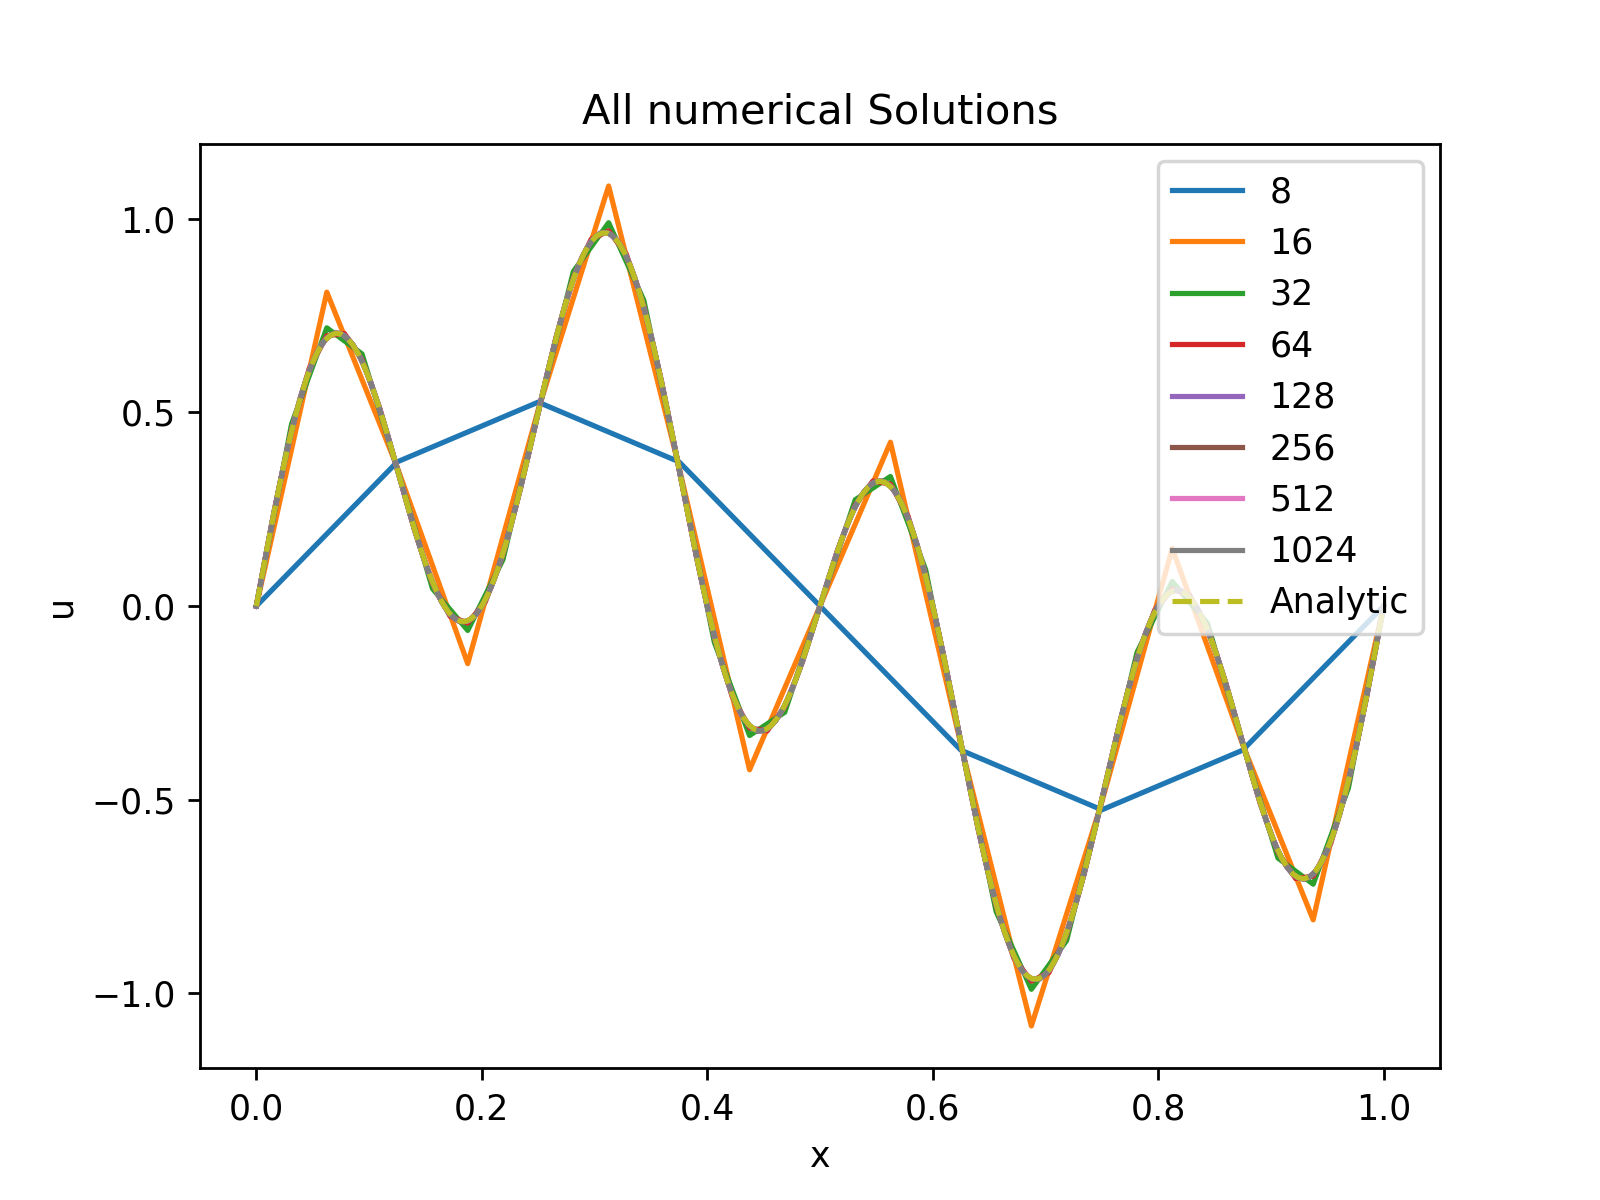
\includegraphics[width=0.75\linewidth]{all_num_solns.png}
    \caption{Numerical solutions for $k=3,\dots10$}
    \label{fig:all-solns}
\end{figure}

\begin{figure}
    \centering
    \begin{subfigure}{0.48\textwidth}
        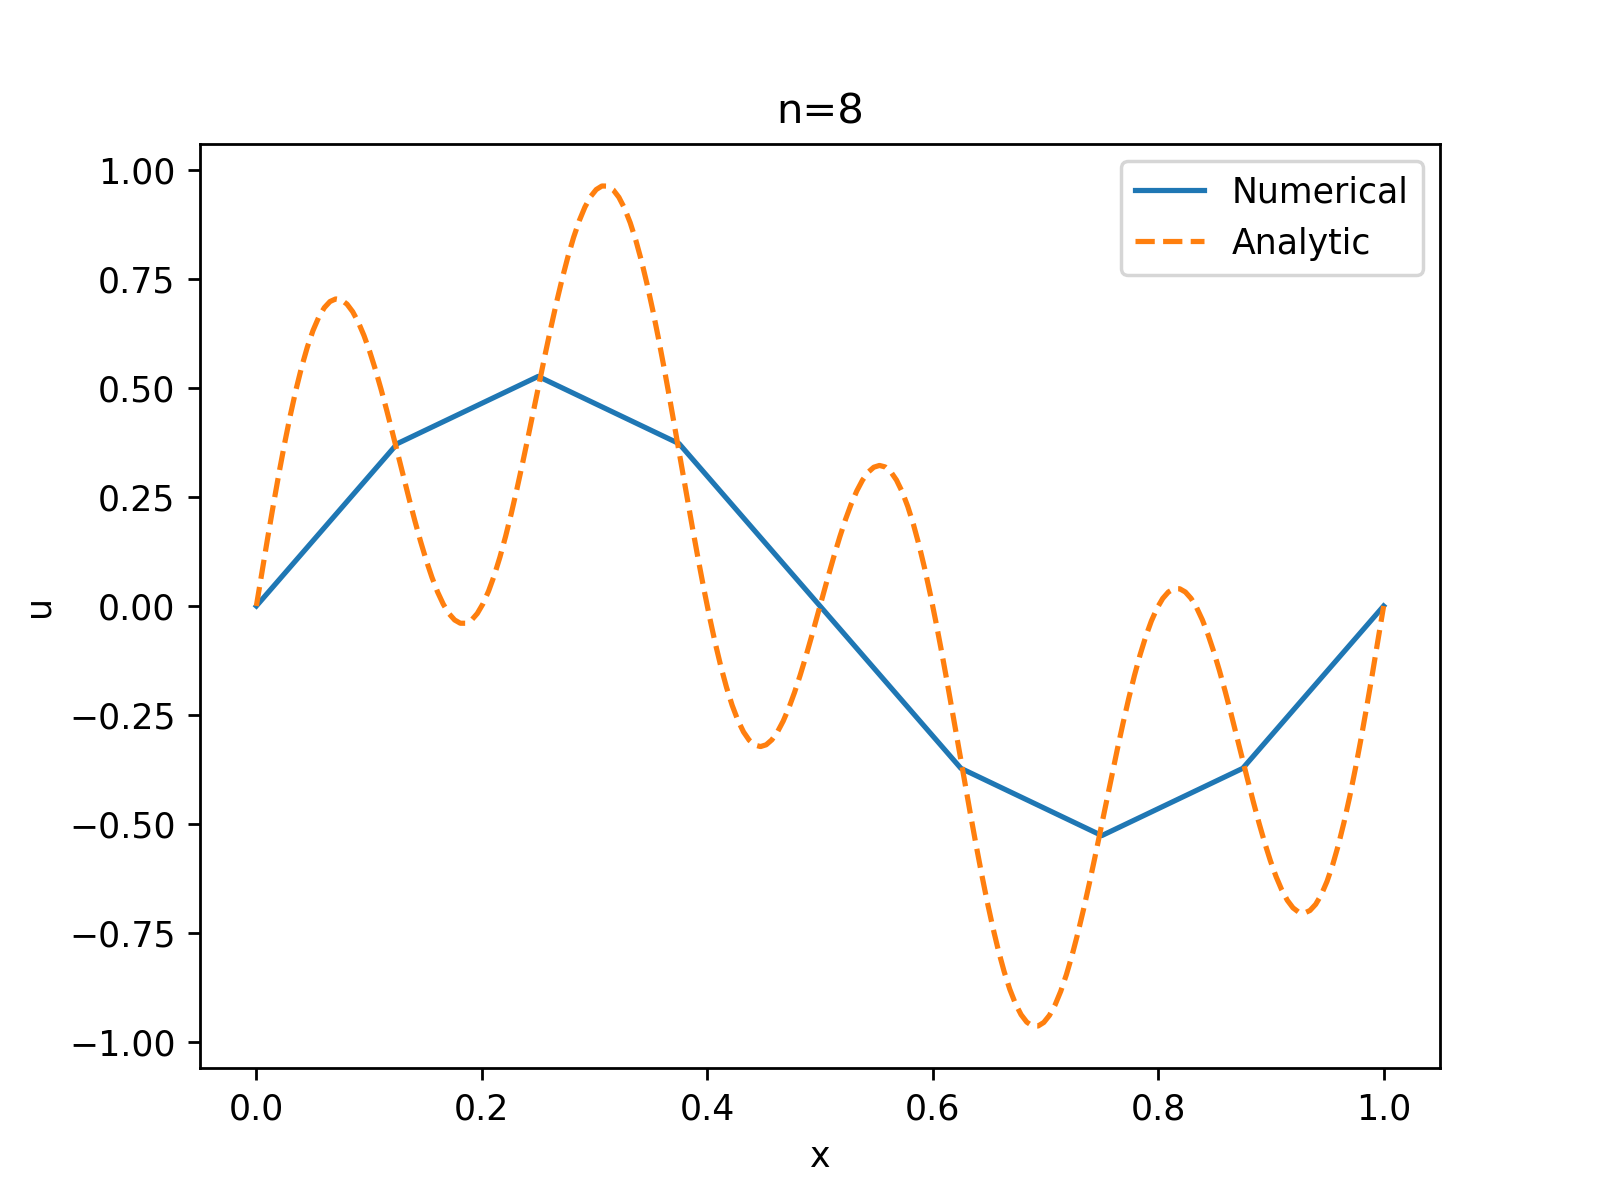
\includegraphics[width=\linewidth]{lowk.png}
        \caption{$k$ = 3}
        \label{}
    \end{subfigure}
    \begin{subfigure}{0.48\textwidth}
        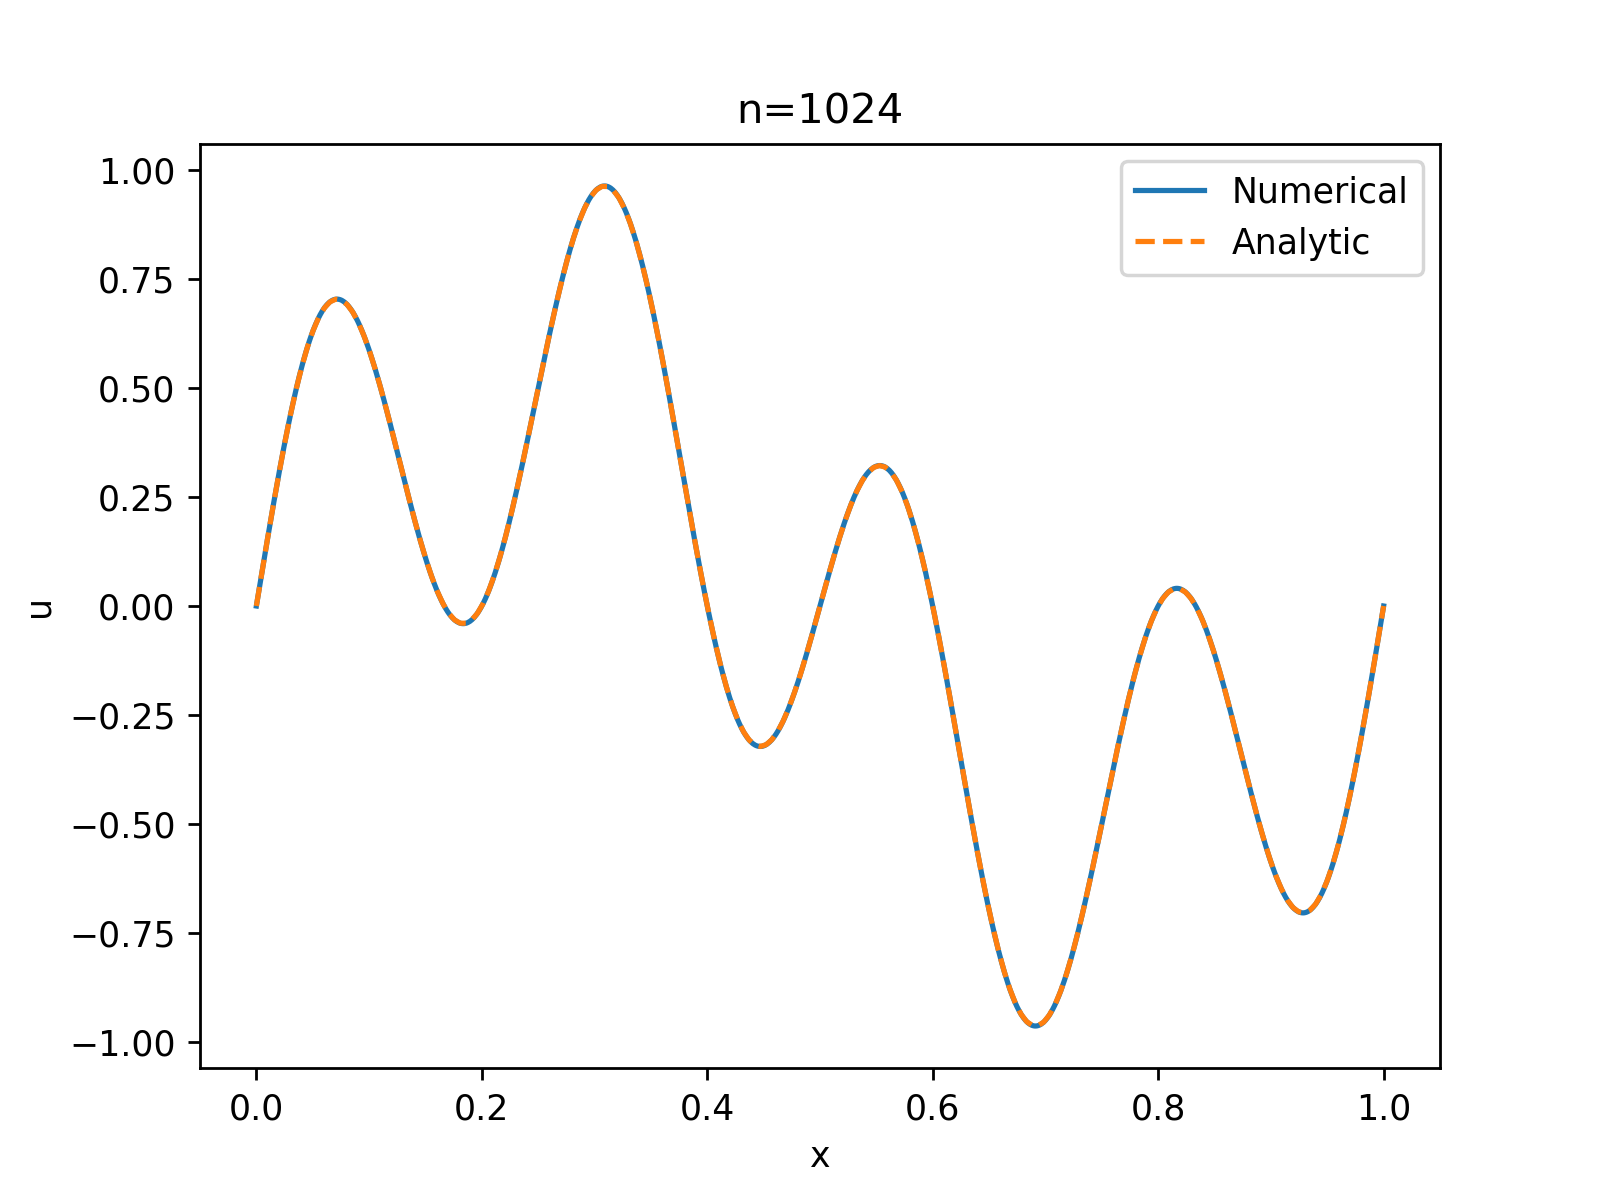
\includegraphics[width=\linewidth]{highk.png}
        \caption{$k$ = 10}
        \label{}
    \end{subfigure}
    \caption{Numerical and analytic solutions for extreme values of $k$. }
    \label{fig:extreme-solns}
\end{figure}

\begin{figure}
    \centering
    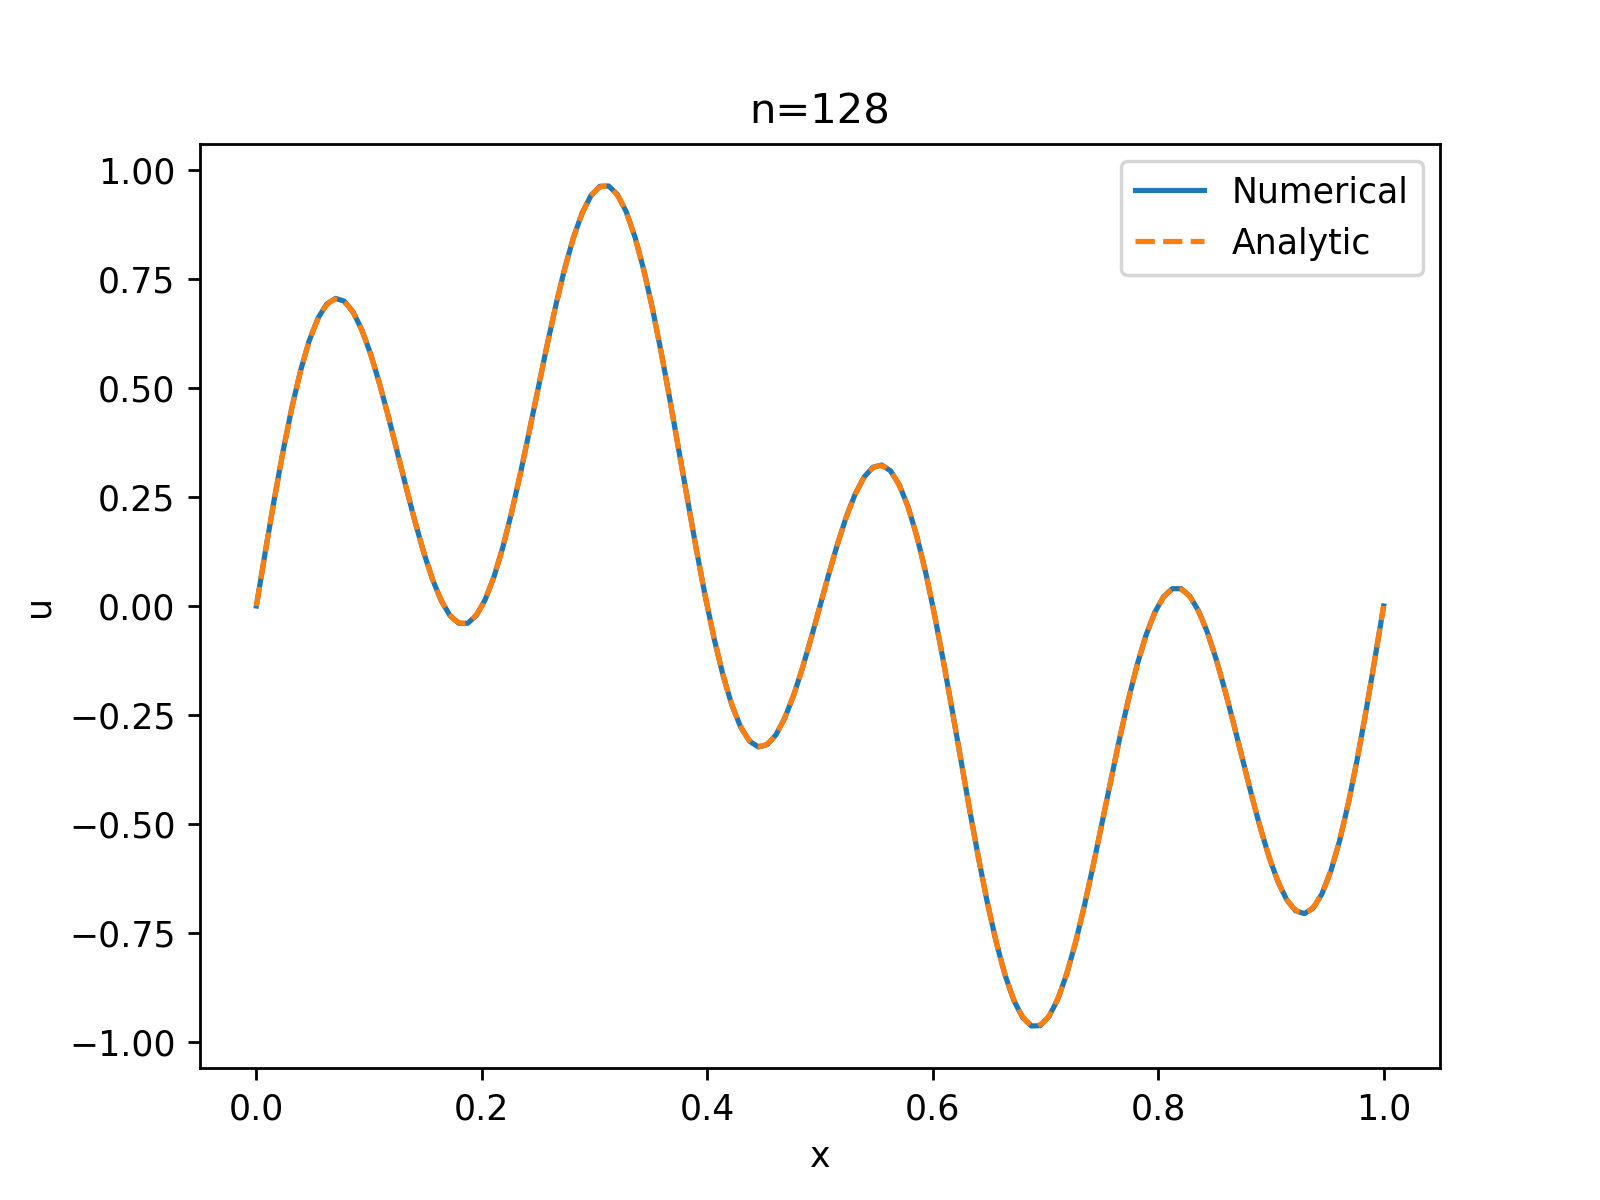
\includegraphics[width=0.48\linewidth]{midk.png}
    \caption{Numerical and analytic solution for intermediate value of k. Note numerical solutions for $k=7, 10$ are visually equivalent}
    \label{fig:mid-soln}
\end{figure}


\subsection{}

The absolute $L_{\infty}$ errors for each solution can be seen in \autoref{fig:abs-error}. The error decreases linearly with $k$. Since $n=2^k$, this indicates logarithmic convergence with regards to $n$, where $E$ is proportional to $-\ln_2(n)$.

It should be noted that the first mesh refinement actually increases the error, since the mesh boundaries roughly coincide with local maxima/minima on the analytical solution, where a linear approximation is a poor model of the real behavior of the solution. The mesh boundaries for $k=3$ fully enclose these local extrema, so their effect is not seen as much as in $k=4$.

The linear convergence is further indicated in \autoref{fig:convergence-ratio}, where the ratio of each error to the error at $k-1$ converges to $0.25$, which again would indicate logarithmic convergence with regards to $n$ -- doubling the number of meshpoints would improve the error by a factor of one-fourth. 


\begin{figure}
    \centering
    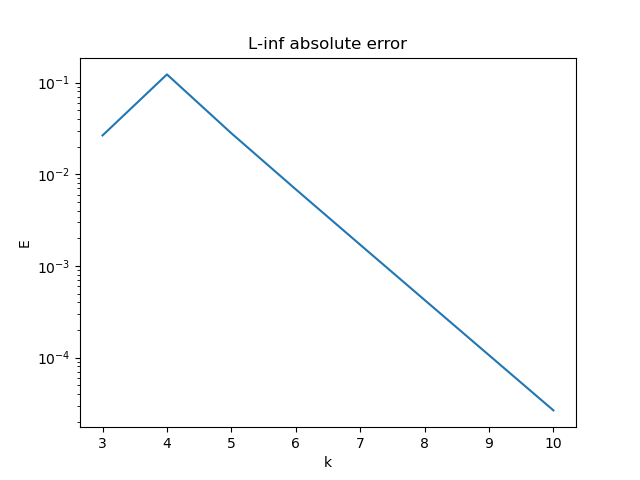
\includegraphics[width=0.65\linewidth]{abs_err.png}
    \caption{Absolute $L_{\infty}$ error for all solutions}
    \label{fig:abs-error}
\end{figure}

\begin{figure}
    \centering
    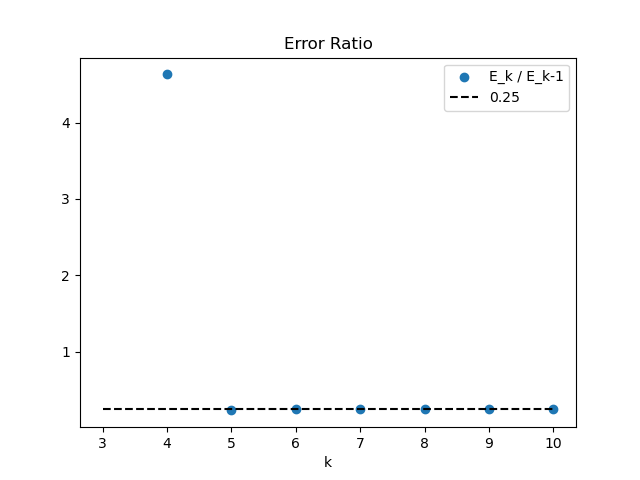
\includegraphics[width=0.65\linewidth]{convergence.png}
    \caption{Convergence ratio. Note $E_{k}/E_{k-1} \rightarrow 0.25$}
    \label{fig:convergence-ratio}
\end{figure}



\bibliographystyle{ieeetr}
\bibliography{references}





\end{document}
